% Filename: path_shade02@tikz_for_teachers.tex
% This code is part of LaTeX with Vim.
% 
% Description: TikZ for teachers is free book about TikZ and Sage.
% 
% Created: 30.03.12 08:10:18 PM
% Last Change: 30.03.12 08:10:28 PM
% 
% Author: Raniere Gaia Costa da Silva, r.gaia.cs@gmail.com
% Organization:  
% 
% Copyright (c) 2010, 2011, 2012, Raniere Gaia Costa da Silva. All rights 
% reserved.
% 
% This file is license under the terms of a Creative Commons Attribution 
% 3.0 Unported License, or (at your option) any later version. More details
% at <http://creativecommons.org/licenses/by/3.0/>.
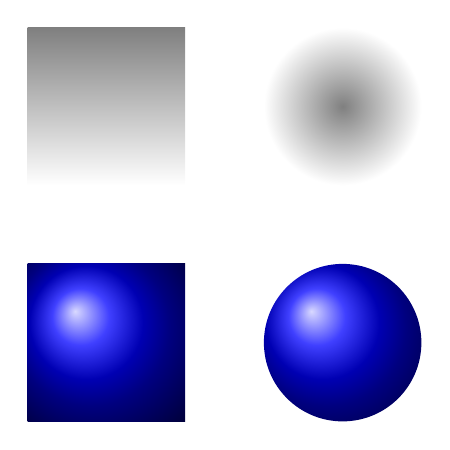
\begin{tikzpicture}
    \path[shade, shading=axis] (0,0) rectangle (2,-2);
    \path[shade, shading=radial] (3,0) rectangle (5,-2);
    \path[shade, shading=ball] (0,-3) rectangle (2,-5);
    \path[shade, shading=ball] (4,-4) circle (1);
\end{tikzpicture}
